\documentclass[a4paper,12pt]{article}
\usepackage{graphicx}
\usepackage{hyperref}
\begin{document}
\title{Chomp
\subsubsection*{Requirements and Specification Document -- Group 6}\subsubsection*{Version 0.1}
}\maketitle
\section*{Project Abstract}
Chomp is a web application that tracks what a person, group, or family eats, and gives nutritional advice, financial suggestions, sustainability ratings, and other meal and dietary statistical analysis.  Chomp provides a more digestable understanding of how our food affects us beyond a simple calorie counter.  By leveraging multiple informational APIs, a wealth of data can be generated from simple meal entries.  Customers use Chomp to gague their daily, weekly, monthly, and yearly progress toward their personal goals, and choose Chomp as their preffered tool because of its variety and wealth of information packed into a convenient and understandable form.  Plans for Chomp include adding a social support network of like-minded users to aid in users' feeling of and drive for success.  The anticipated revenue stream for Chomp will be in-app addvertisements that target a given user.

Our github location is \url{http://github.com/hedekar/chomp}
\section*{Customers}
\subsubsection*{Weight Loss}
This customer uses Chomp to keep a daily count of their calories and specific nutritional information to assist them in losing weight.  See Appendix 1 for the user persona of Boris Chetznekov for further info.
\subsubsection*{Family Nutrition}
This customer uses Chomp to track how nutritious her family meals are and what deficiencies in the diet may need to be addressed.  She is also very concerned with meal cost.  See Appendix 1 for the user persona of Susan Montgomery for further info.
\subsubsection*{Body Builder}
This customer uses Chomp to monitor his body's nutrition levels as he prepares for body building competitions.  He lives with two roommates who also work out but not to the same level of competitiveness, but they all share groceries.  See Appendix 1 for the user persona of Chet Reist for further info.
\section*{Competitive Analysis}
Many other meal-tracking services already exist.  Some have multiple million downloads and users.  The majority of these however are very specific in scope, with only calories being counted or with a focus on reporting all the nutritional numbers at once.  The large majority of these applications are targeting weight loss customers, and not an everyday user.

Both web applications and mobile applications have been developed in this field.  Some specific competitors include: \begin{list}{•}{•}
\item \textbf{Noom Coach} -- A semi-free app that counts calories and tracks weight of the user.  The paid version allows for community sharing of progress and chatting amongst similar-goaled users.
\item \textbf{MyFitnessPal}
\item \textbf{Lifesum}
\item \textbf{FatSecret}
\item \textbf{My Food Diary}
\end{list}
\section*{User Stories}
% to include in each story: Name/Description, Actors/Personas, Precondition/trigger, Actions/Post Condition, Acceptance Criteria, Tests
\subsection{User Accounts}
\textbf{Personas involved:} All
\subsubsection{Registration}
\textbf{Precondition:} An unrecognized or not-logged in user visits our frontpage.\\
\textbf{Actions:} A user is greeted with an interface requesting to register.  Options for both Google and Facebook account linkage (via their account APIs) will be presented as well as a manual entry field for e-mail and password. \begin{list}{•}{•}
\item Google's API registration will request the user for their google e-mail and password.  After this is submitted, the
\item Facebook's API registration will request the user for their Facebook e-mail and password.  This will then re-direct to a facebook window that asks the user to agree for us to get certain 
\item Manual entry process will request first name, last name, username, and e-mail.  This will be followed up by sending the user's e-mail a confirmation message in which a unique activation link will be sent.  The process will end at a page instructing users to look for their e-mail link that will allow them to finish setting up their account.
\end{list}
After registration completion, the system will send the user directly to the Account Setup stage.\\
\textbf{Test/Postcondition:} A new account should be attempted to be created via google, facebook, as well as manually and the database should register all of the user's submitted information.  To check, developers can access the database directly to see the adition.
\subsubsection{Account Setup}
\textbf{Precondition:} Either the user's account has freshly been registered, or they have clicked on the 'Account Settings' button of their user profile.\\
\textbf{Actions:} If the account is already setup, the dialogue will present the setup items as an editable listing rather than sequential prompts.  A dialogue will ask the user about the following items\begin{list}{•}{•}
\item Number of users to track (along with their usernames if they're also Chomp users)
\item Birthdate (of primary user and each non-Chomp user)
\item Current weight (of primary user and each non-Chomp user)
\item Height (of primary user and each non-Chomp user)
\item Personal priority ranking (eg. sustainability, carbohydrate intake, finances, etc..)
\end{list}
Once all of this information is submitted, the user's account will be updated and the desired statistics will take priority in the nutrition and value tracking interface.\\
\textbf{Test/Postcondition:} 
\subsubsection{Login}
\textbf{Precondition:}\\
\textbf{Actions:}\\
\textbf{Test/Postcondition:}
\subsubsection{Logout}
\textbf{Precondition:}\\
\textbf{Actions:}\\
\textbf{Test/Postcondition:}
\section*{User Interface Requirements}
There are four major sections of our user interface that should be considered critical to the application's success.
\begin{list}{•}{•}
\item \textbf{Meal Entry Dialogue}  This dialogue should allow entry for time of meal, contents of meal, and portion of meal.
\item \textbf{Personal Nutritional \& Value Tracking}
\item \textbf{Suggested Meal Listing}
\item \textbf{Community Support Feed}
\end{list}
\newpage 
\section*{Appendix 1 - User Personas}
\subsection*{Boris Chetznekov}

\includegraphics[scale=0.3]{Boris.jpg}
Age: 65\\
\subsection*{Susan Montgomery}

\includegraphics[scale=0.23]{Susan.jpg}
Age: 32\\
\subsection*{Chet Reist}
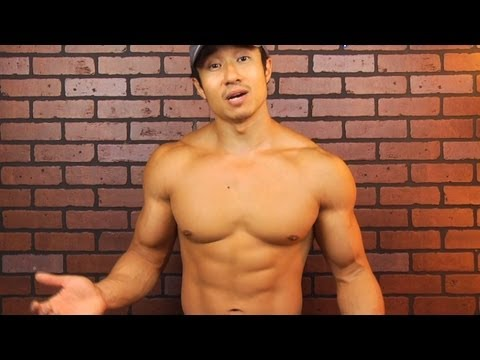
\includegraphics[scale=0.38]{Chet.jpg}
Age: 21\\
\end{document}